\documentclass{article}


% Essentials and Formatting
\usepackage[utf8]{inputenc}                          % encodes unicode stuff
\usepackage{graphicx}                                % helps make pretty pictures
\usepackage{multicol}                                % multicolumn/multirow cells in tables
\usepackage{dcolumn}                                 % Align table columns on decimal point
\usepackage[table,usenames,dvipsnames]{xcolor}       % extra colors (i like ForestGreen)
\usepackage{xparse}                                  % make new commands i think
\usepackage[margin=1in]{geometry}                    % controls document shape/size
%\usepackage[backend=biber, sorting=nyt]{biblatex-chicago}              % for bibliographies
\usepackage{calligra}                                % solely for Griffiths r
\usepackage{fancyhdr}                                % control of headers and footers
\usepackage{lastpage}                                % not entirely sure tbh
\usepackage{titlesec}                                % control of section heading formatting
\usepackage{listings}                                % for formatting code nicely


% Math and Science
\usepackage{bbm, bm}                   % "blackboard bold" for real numbers
\usepackage{amsmath}                   % makes typing math stuff easier
\usepackage{amsthm}                    % makes typing actual math stuff easier
\usepackage{siunitx}                   % makes typing units easier
\usepackage{derivative}                % makes typing derivatives easier
\usepackage[version=4]{mhchem}         % makes typing chemistry easier


% Graphs, Tables, and Figures
\usepackage{tikz}                      % pictures
\usepackage{pgfplots}                  % pretty graphs
\usepackage{pgfplotstable}             % formatting options for tables
\usepackage{adjustbox}                 % puts a box around things that are too big and makes them smaller
\usepackage{caption}                   % caption stuff for tables and plots
\usepackage{subcaption}                % same but for subtables and subfigures
\usepackage{csvsimple}                 % easy compatability with comma separated value files


% Citations and references
\usepackage{natbib}                                  % for STEM, uses bibtex NOT biber
\setcitestyle{square, super}
%\usepackage[backend=biber, sorting=nyt]{biblatex}   % for basically only Music History
\usepackage{bookmark}                                % bookmarks. includes hyperref
\usepackage{cleveref}                                % automatically determines the kind of reference


% Package configuration
\hypersetup{colorlinks=true, allcolors=blue}
\sisetup{per-mode = fraction, list-final-separator = {, and }, group-digits=integer, fraction-function=\tfrac}
\pgfplotsset{compat=1.18}
%\addbibresource{sources.bib} % Remember to run biber 'filename' in the terminal if using
%\bibliography{sources} % Move to end of file when using natbib
\fancypagestyle{firststyle}
{
    \fancyhf{}
    \fancyhead[L]{PHYS 4023 $-$ Mystery Data}
    \fancyhead[R]{Joseph Temple}
    \renewcommand{\headrulewidth}{0pt} % removes horizontal header line
    \setlength{\headheight}{26.0pt}

    \fancyfoot[C]{\thepage}
}


% The actual document
\begin{document}

\begin{titlepage}
    \begin{center}
        \vspace*{1cm}
 
        \huge
        \textbf{Project 1}
 
        \Large
        Fitting to Experimental Data with \verb|scipy.optimize|
             

        \vfill

        \textbf{Joseph Temple}
        
 
        \vfill

        Arkansas Tech University \\
        PHYS 4023 Computational Physics \\
        September 26, 2025  
    \end{center}
 \end{titlepage}

\pagestyle{firststyle}


\section{Introduction}

Experimental data is often wrought with deviation from theoretically predicted behavior. Be it through
human mistakes, imprecise measurement tools, or the slightest shift in environment, it is nigh-on-impossible
to perform an experiment full unperturbed. As such, it behooves us to have computational tools to deal with
such imperfections. One such tool is \emph{curve fitting}, in which we define an abstract functional form
(either through theory or observation) to be fit to the experimental data. The ubiquitous Python module
\verb|scipy| provides an implementation of curve fitting, which performs a least-squares optimization,
minimizing the error between a fit curve and the experimental data by adjusting the parameters defining
the functional form.

In this project, we were provided with three experimental datasets without context of the experiments
from which they were generated. After deciding upon appropriate functional forms for each, we
were tasked with fitting curves to each dataset, analyzing the accuracy of said curve fits, and
deciphering plausible physical phenomena each represents. To do so required a healthy use of
\verb|matplotlib|, $\verb|scipy.optimize.curve_fit()|$, \verb|pandas|, and $\verb|numpy|$. 
All computations were performed in Jupyter notebook.

\section{Initial Analysis}

Each of the three datasets was provided as a Comma-Separated Values file: \verb|Dataset_A.csv|, 
\verb|Dataset_B.csv|, and \verb|Dataset_C.csv|. Each file has two columns, one labeled $t$ and one
labeled $f(t)$. Reading in each as a \verb|pandas| DataFrame and splitting the two columns
into separate 1-dimensional \verb|numpy| arrays (named \verb|X_t| and \verb|X_ft| respectively, 
for $\verb|X| \in \{\verb|A|,\verb|B|,\verb|C|\}$), we performed an initial inspection of the datasets
by plotting them with \verb|matplotlib|. See \Cref{fig:read} and \Cref{fig:plot1} in \Cref{sec:appendix}
to see the Python code. In \Cref{fig:init}, we have plotted each as individual 
points, and then connected said dots to create a continuous curve.

\begin{figure}[ht]
    \centering

    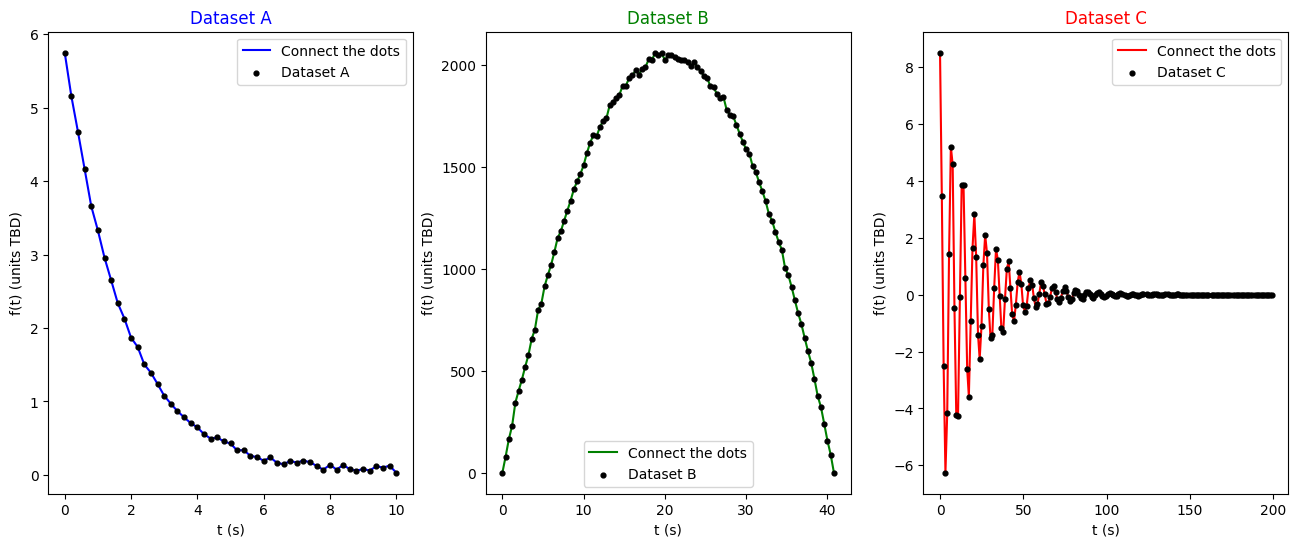
\includegraphics[width=0.9\textwidth]{../figures/init.png}

    \caption{Initial visualization of three datasets.}

    \label{fig:init}
\end{figure}

By inspection, we assume Dataset A to be an exponential decay function, Dataset B to be a parabola,
and Dataset C to be a damped oscillator (an exponentially decaying sinusoid). As such, we define three
functions: $f_A(t) = ae^{-bt} + c$, $f_B(t) = at^2 + bt + c$, and $f_C(t) = be^{-at}\sin(ct + d)$.
See \Cref{fig:func} in \Cref{sec:appendix} for code defining these functions.
In testing, we also analyzed a variant $f_C$ using a linear combination of $\sin(ct)$ and $\cos(ct)$ rather
than the phase shift--this is the source of the non-alphabetical variable ordering as that came
first and this ordering was chosen to match--but we find the phase-shifted 
version to be more easily interpretable. 

\section{Curve Fitting}

The process of curve fitting is then a pretty straightforward process, thanks to \verb|scipy|. Calling
the function \verb|scipy.optimize.curve_fit(f_X, X_t, X_ft)| with parameters of the function
to be fit, the time series data array, and the dependent variable data array returns two useful objects
for us. First is a numpy array containing the fitting parameters $a$, $b$, $c$, and possibly $d$ 
(one of which we will refer to generally as $y$) fit to the values that most closely model the experimental 
data. Second is a symmetric covariance matrix, of size $p \times p$ where $p$ is the number of fitting parameters, 
in which the diagonal terms give the variance $\sigma_y^2$ (squared uncertainty) in each parameter. The 
off-diagonal terms give covariances $\sigma_{y_1}\sigma_{y_2}$, how correlated pairs of variables are. 
In each case, a good fit is indicated by low numbers; low variance means our parameters neatly fit to the data, 
and low covariance means the fitting parameters are independent of one another, which we expect to be the case.
See \Cref{fig:fitcode} in \Cref{sec:appendix} for the code of curve fitting.

We'll start with the first return of the \verb|curve_fit| function: the parameters themselves. After
fitting, we found the following functional forms, with each parameter rounded to 3 decimal places:
\begin{align*}
    f_A(t) &= 5.733e^{-0.566t} + 0.049 \\
    f_B(t) &= -4.902t^2 + 200.062t + 3.995 \\
    f_C(t) &= 7.813e^{-0.048t} \sin\left(0.923t + 1.543\right)
\end{align*}

Then, we can plug each array \verb|X_t| into the corresponding functional form with the fitted parameters 
to graph our fitted model. Doing so for each functional form (including the later decided-against linear 
combination version of $f_C$) gives \Cref{fig:fit}. See \Cref{fig:plot2} in \Cref{sec:appendix} for the code.

\begin{figure}[ht]
    \centering

    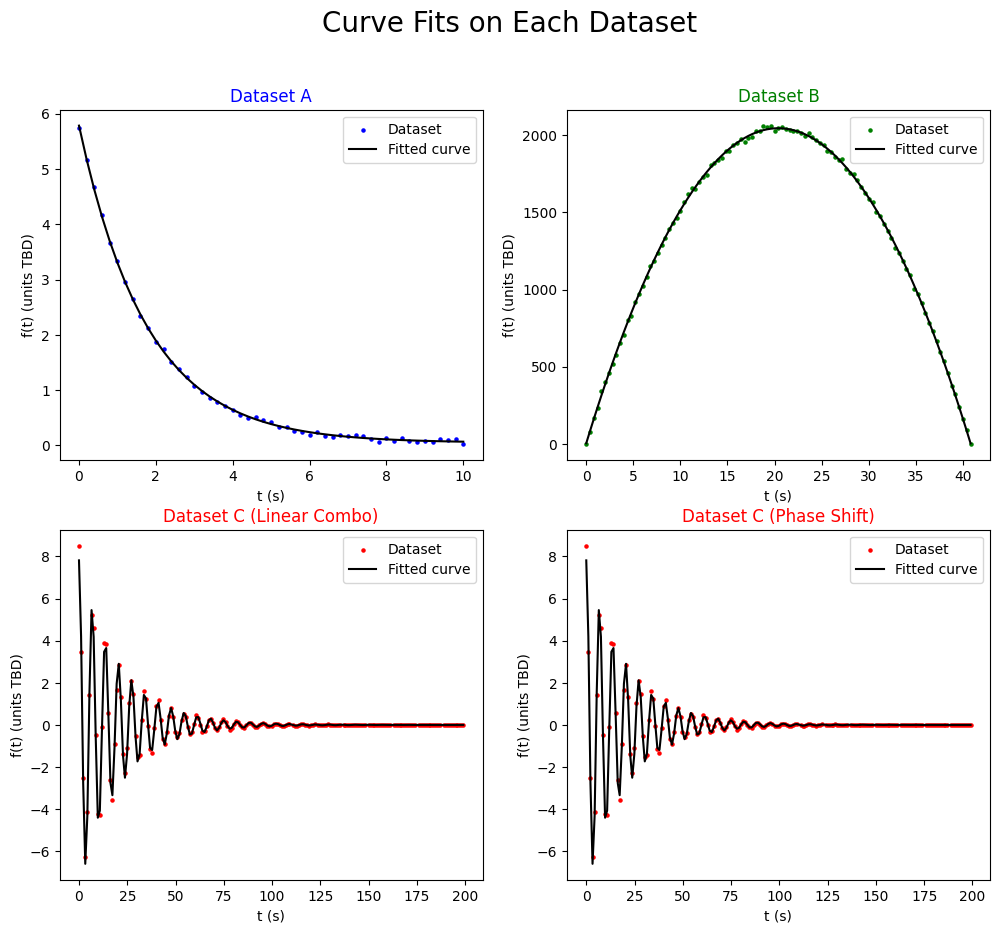
\includegraphics[width=0.75\textwidth]{../figures/fit.png}

    \caption{All three datasets with fitted curves overlaid.}

    \label{fig:fit}
\end{figure}

\section{Uncertainty Analysis}

As we see, no datapoints are particularly distant from their respective curve, meaning the fits performed 
very well. Of course, the covariance matrix previously discussed provides us with quantitative tools to
analyze beyond mere visual inspection. The full covariance matrices are given in 
in \Cref{fig:cov} of \Cref{sec:appendix}, but as discussed prior the most important values are the variances 
along the diagonal. See \Cref{fig:fit_num} below for the fit values of the parameters with uncertainty 
determined by taking the square root of each variance value.

\begin{figure}[ht]
    \centering

    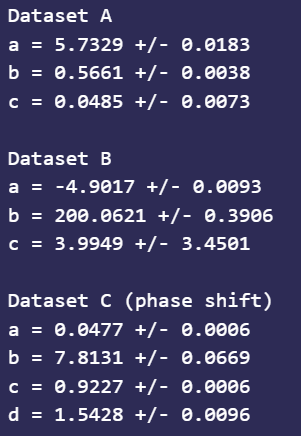
\includegraphics[width=0.3\textwidth]{../figures/param_with_stddev.png}

    \caption{All three datasets with fitted curves overlaid.}

    \label{fig:fit_num}
\end{figure}

We see that nearly every parameter has uncertainty on the verge of negligibility, 
two or more orders of magnitude less than the value itself, with the notable
exception of the $c$ parameters of Dataset \verb|A| and especially of Dataset \verb|B|. Both of these
represent $y-$intercepts, the value of $f_X(t)$ when $t=0$, which is a notoriously sensitive
parameter. Additionally, in Dataset \verb|B| the values $f_B(t)$ are very far from 0 when $t$ is far
from zero, meaning slight differences in the other parameters can change $c$ somewhat drastically.
Indeed, we see in \Cref{fig:cov}, the off-diagonal terms of the covariance
matrix for parameter $c$ (along the third row and third column) are orders of magnitude
greater than the other off-diagonal entries, meaning that there is some coupling between $c$ and
those other parameters. Overall though, we see that the variance is quite low and our curve fit
rather accurately maps to the data.

\section{Physical Interpretation}

\subsection{Dataset \texttt{A}}

A common exponential decay in physics is the number of particles in a sample in a radioactive material. 
A typical way to write this would be $N(t) = N_0e^{-\lambda t}$. Since our fit parameter has 
$c \approx 0$, it is fair for us to ignore that term and let $a = N_0$ and $b = \lambda$.

Now, it wouldn't make physical sense to start with $5.733$ particles, so I'll take the units of $N_0 = a$ to be, 
say ``mega-particles'', where $5.773 \text{ megaparticles} = 5.773 \times 10^{6} \text{ particles}$, rounding
that down to the nearest integer. $\lambda = b$ is then the decay constant, which has physical units of 
inverse time.
\begin{align*}
    f_A(t) &= \left(5732880 \text{ particles}\right)e^{-\left(\qty{0.566}{\second^{-1}}\right)t}
\end{align*}

\subsection{Dataset \texttt{B}}
A common parabolic shape like this in physics would be the trajectory of a projectile $y(t) = 
-\frac{1}{2}gt^2 + v_0t + y_0$. So here we have $a = -\frac{1}{2}g$, with units of 
$\unit{\meter\per\square\second}$, $b = v_0$ with units of $\unit{\meter\per\second}$, and $c = y_0$ 
with units of $\text{m}$. Calculating $g$ from our $a$ fit we find $g = \qty{9.803}{\meter\per\second\squared}$,
and taking the other coefficients directly, we find the following curve fit function:
\begin{align*}
    f_B(t) &= \left(\qty{9.803}{\meter\per\square\second}\right)t^2 + 
    \left(\qty{200.062}{\meter\per\second}\right)t + \left(\qty{3.995}{\meter}\right)
\end{align*}

\subsection{Dataset \texttt{C}}
Plenty of things could be an underdamped oscillator. I'll go with the prototypical example of a damped mass 
spring. The physical meaning of the parameters takes a fair bit more work here, so I'll actually do the 
derivation. Say we have a mass $m$ (in kg) oscillating on a spring with spring constant $k$ (in 
$\unit{\newton\per\meter}$ or $\unit{\kilo\gram\per\square\second}$), and damping constant $\beta$ 
(in $\unit{\kilo\gram\per\second}$ or $\unit{\newton\second\per\meter}$)

\begin{align*}
    m\ddot{x} + \beta\dot{x} + kx &= 0 \\
    \ddot{x} + \frac{\beta}{m}\dot{x} + \frac{k}{m}x &= 0 \\
    \ddot{x} + 2\gamma\dot{x} + \omega_0^2x &= 0 \qquad \text{ where } \gamma = \frac{\beta}{2m} \text{ and } \omega_0 = \sqrt{\frac{k}{m}}
\end{align*}
This is underdamped when the discriminant of the characteristic equation is negative. That is, if 
$\gamma^2 < \omega_0^2$, and the solution involves the damped frequency 
$\omega_d = \sqrt{\omega_0^2 - \gamma^2}$. That solution is this:
\begin{align*}
    x(t) &= Be^{-\gamma t}\sin\left(\omega_d t + \phi\right)
\end{align*}

What we notice is that coefficient out front (our $b$) is the maximum amplitude of the oscillation for $t=0$. 
So that would be $b = B = \qty{7.813}{\meter}$. The exponential decay factor is $a = \gamma =  
\qty{0.048}{\second^{-1}}$, 
and the damped frequency is $c = \omega_d = \qty{0.923}{\radian\per\second}$. Now, what's interesting about 
the phase is that it is \emph{very} close to $\frac{\pi}{2}$. We see that $2d \approx 3.09$, which 
means $d$ itself is only a degree or 2 away from being $\frac{\pi}{2}$. We can use that to transform it 
into a $\cos$ function, since $\sin(\omega t + \frac{\pi}{2}) = \cos(\omega t)$. This brings our final
functional form to the following:
\begin{align*}
    f_C(t) &= \left(\qty{7.813}{\meter}\right)e^{-\left(\qty{0.048}{\second^{-1}}\right)t}
    \cos\left(\left(\qty{0.923}{\radian\per\second}\right)t\right)
\end{align*}

\section{Conclusion}
Curve fitting is a computational method by which a mathematical function is fit to an experimental
dataset such that the squared distance between the curve and the data is as close to zero as possible.
We applied the \verb|scipy| implementation of this algorithm to determine the physical process
measured in each dataset. In general, each fit performed very well--closely hugging the points with
rather low variance--meaning our experimental data was very neat and our fitting was rather precise.
Analyzing the results of eachd we were able to ascribe physical meaning to each
fitted parameter. As such, we consider the Dataset Mystery to be succinctly resolved.

\section{Appendix: Code}
\label{sec:appendix}

The full code is provided at \url{https://github.com/josephtemple/JT_PHYS4023} under the \verb|/Project 1/|
directory. Indeed, one could not locate the directory of this PDF wtithout passing the code
along the way blocks of code and certain outputs are also provided below.

\begin{figure}[ht]
    \centering

    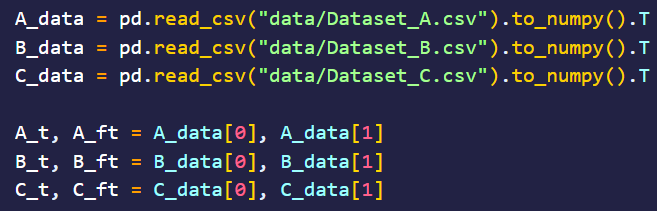
\includegraphics[width=0.76\textwidth]{../figures/read_code.png}

    \caption{Code to read \texttt{csv} files into pandas dataframes and convert them to numpy arrays.}

    \label{fig:read}
\end{figure}


\begin{figure}[ht]
    \centering

    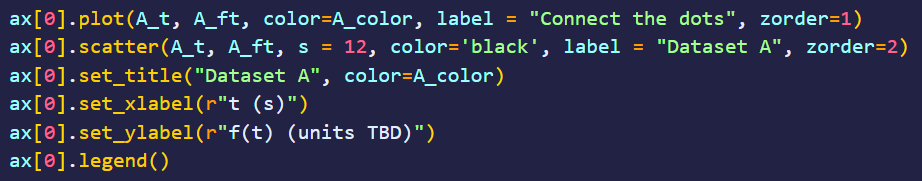
\includegraphics[width=0.76\textwidth]{../figures/plot_code.png}

    \caption{Initial \texttt{matplotlib} code for visualizing raw datasets.}

    \label{fig:plot1}
\end{figure}


\begin{figure}[ht]
    \centering

    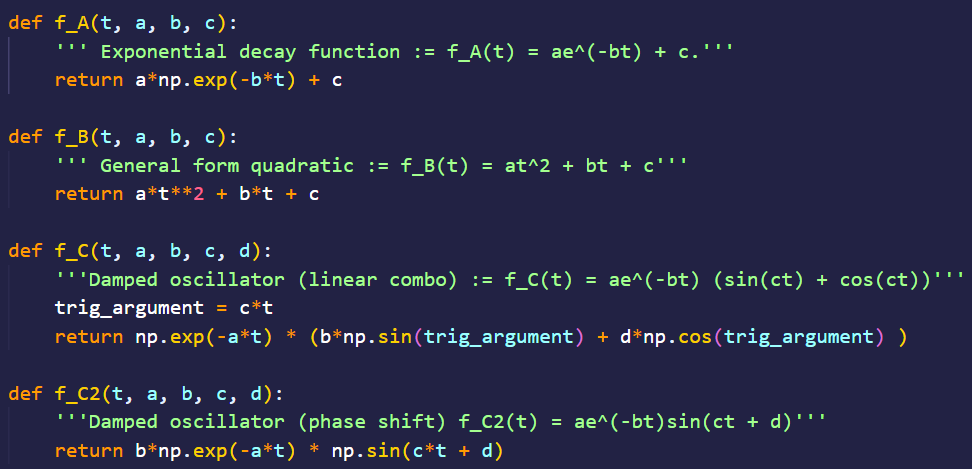
\includegraphics[width=0.76\textwidth]{../figures/func_code.png}

    \caption{Python functions defining mathematical models of each dataset.}

    \label{fig:func}
\end{figure}

\begin{figure}[ht]
    \centering

    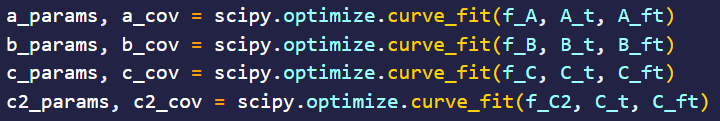
\includegraphics[width=0.76\textwidth]{../figures/fit_code.png}

    \caption{Curve fitting to define parameter arrays and covariance matrices.}

    \label{fig:fitcode}
\end{figure}


\begin{figure}[ht]
    \centering

    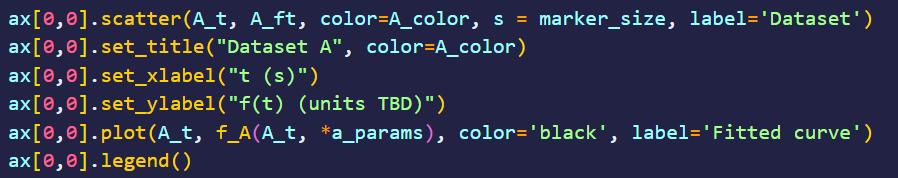
\includegraphics[width=0.76\textwidth]{../figures/plot2_code.png}

    \caption{\texttt{matplotlib} code for visualizing curve fits overlaid with raw data.}

    \label{fig:plot2}
\end{figure}


\begin{figure}[ht]
    \centering

    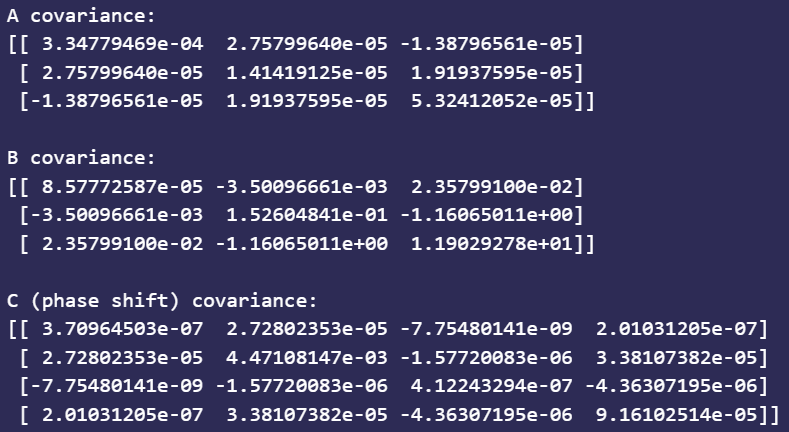
\includegraphics[width=0.76\textwidth]{../figures/cov_code.png}

    \caption{Covariance matrix of primary three curve fits.}

    \label{fig:cov}
\end{figure}



\end{document}